\documentclass[a4paper]{article}
\usepackage[english]{babel}
\usepackage{multicol}
\usepackage{amsmath}
\usepackage{amsfonts}
\usepackage{amssymb}
\usepackage[font=scriptsize]{caption}
\usepackage{parskip}
\usepackage[a4paper, margin= 1in ,total={6in, 8in}]{geometry}
\usepackage{titling}
\usepackage{subcaption}
\usepackage{float}
\usepackage{placeins}
\usepackage{graphicx}

\parskip = 6pt plus 2pt minus 2pt
\setlength{\droptitle}{-2cm}

\title{HW1- Computer Simulation II}
\author{Schewtschik, Guilherme  (3748052)}
\date{\today}

\begin{document}
\maketitle

\section{}

We can calculate the autocorrelation time using the magnetization, plotting it in a log scale we get:

\begin{figure}[H]
    \centering
    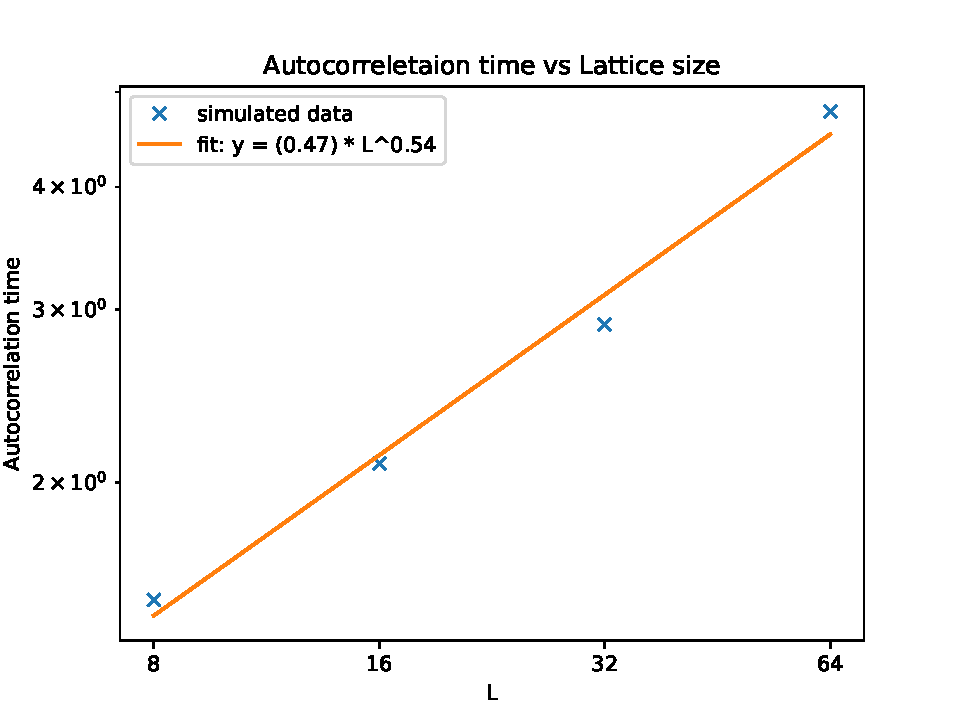
\includegraphics[width=0.65\linewidth]{figures/autocorrelation.pdf}
    \caption{Autocorrelation time for the clusters}
    \label{fig:placeholder}
\end{figure}

To convert this into units of lattice sweeps we use:
\begin{equation}
\tau_{\text{sweep}} = \tau_{\text{cluster}} \cdot \frac{\langle s \rangle}{L^2}.
\end{equation}

Where $\langle s \rangle$ is the average cluster size. Plotting in log scale we get:

\begin{figure}[H]
    \centering
    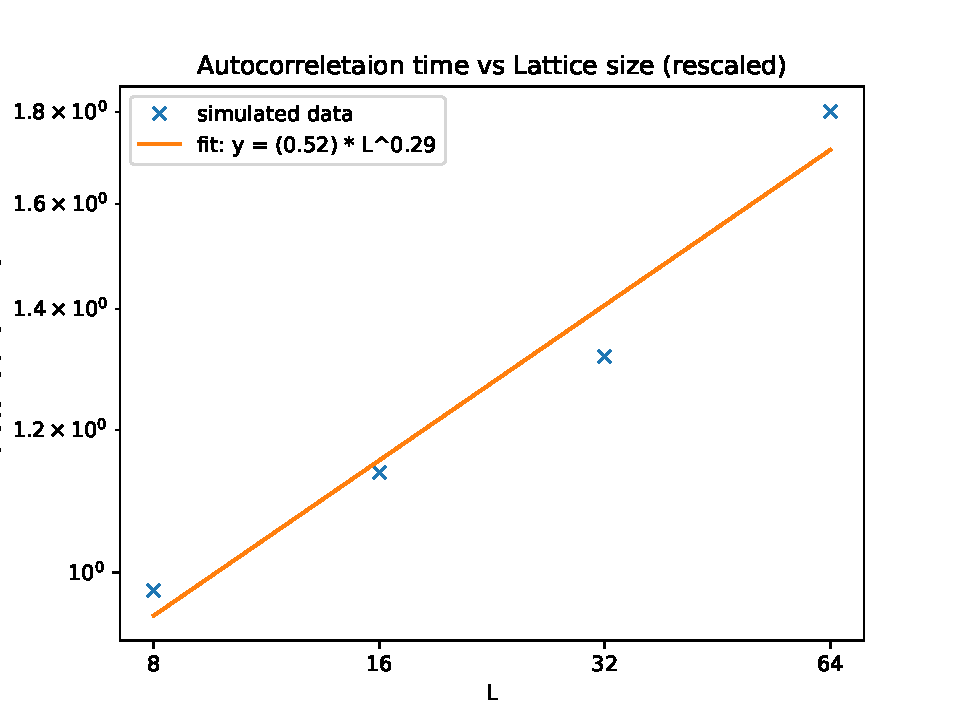
\includegraphics[width=0.65\linewidth]{figures/autocorrelation_scale.pdf}
    \caption{Rescaled correlation time}
    \label{fig:placeholder}
\end{figure}

So we can see:
\[
\tau \propto L^{0.29}
\]
This is significantly less then the autocorrelation time of the Metropolis algorithm $\tau \propto L^{2.17}$, but still 
a bit larger then the expected amount for the Wolff algorithm $z \approx 0.13$.


\section{}
Calculating the value of $\chi$ we can clearly see the peaks around the critical temperature:

\begin{figure}[H]
    \centering
    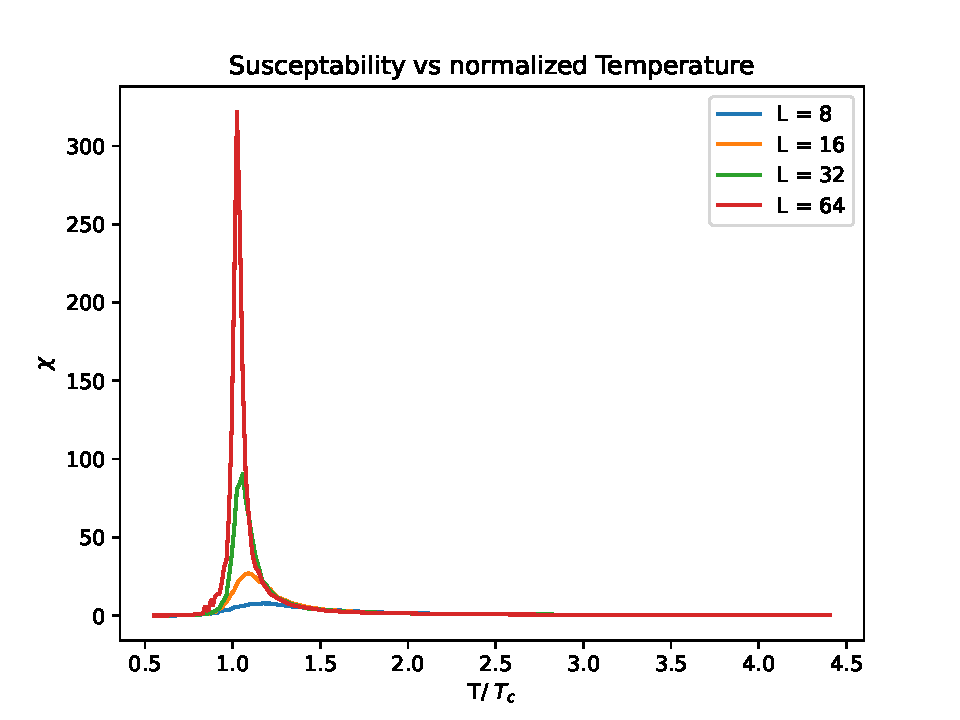
\includegraphics[width=0.65\linewidth]{../../HW1/tex/plots/chi.pdf}
    \caption{$\chi$ values}
    \label{fig:placeholder}
\end{figure}

Taking the maximum of $\chi$ and plotting it against the lattice size $L$, we can see the relation between them scales by a power law:

\begin{figure}[H]
    \centering
    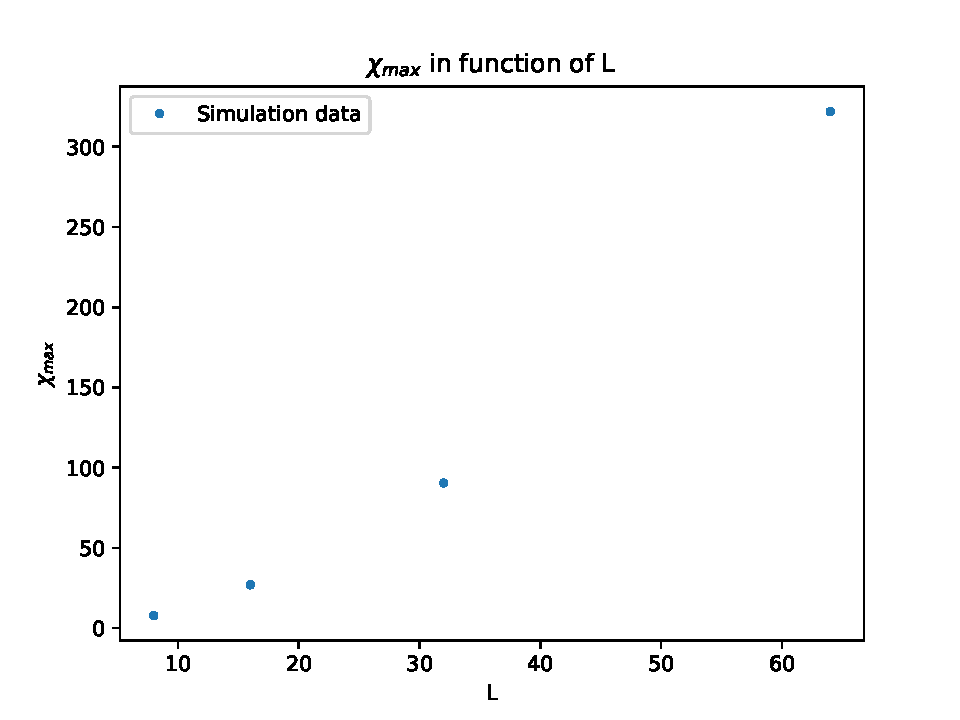
\includegraphics[width=0.65\linewidth]{../../HW1/tex/plots/chi_max.pdf}
    \caption{$\chi$ in function of $L$} 
    \label{fig:placeholder}
\end{figure}
\newpage
For us to test the finite-size scaling Ansatz, we first need to make some adjustments, instead of using the given formula we shall work in log space:

\begin{equation}
    ln(\chi) = \frac{\gamma}{\nu}ln(L) + c
\end{equation}

Where $c$ is a proportionality constant. Using this equation and 
fitting a line we can find the values for $\gamma/ \nu$ and $c$.

\begin{align}
    \frac{\gamma}{\nu} = 1.783169... \quad c = - 1.65374
\end{align}
    
\begin{figure}[H]
    \centering
    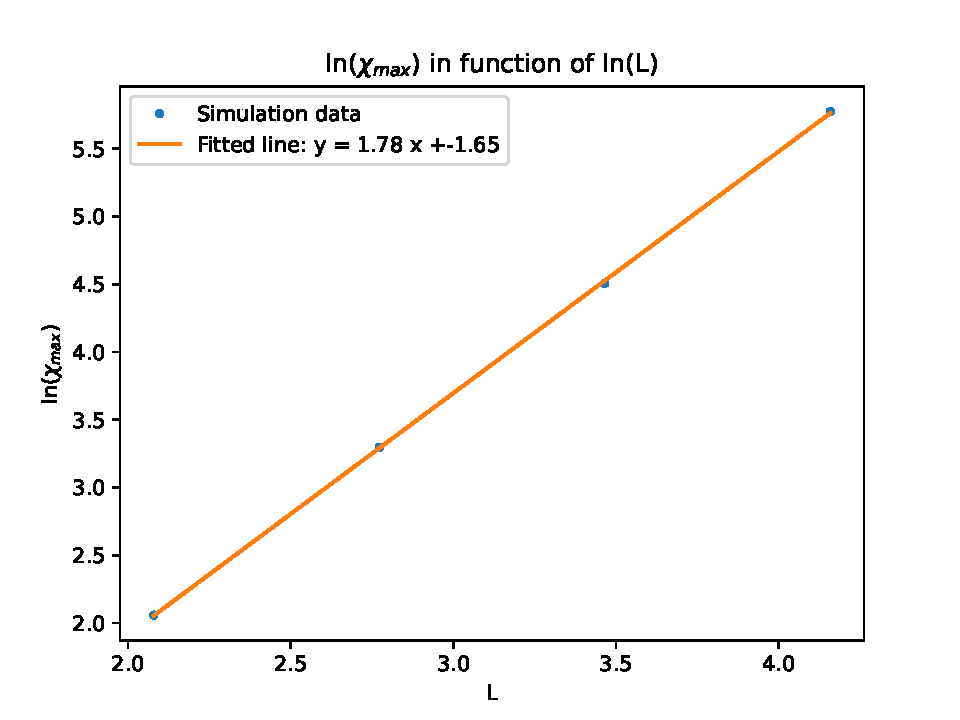
\includegraphics[width=0.7\linewidth]{../../HW1/tex/plots/ln_chi.pdf}
    \caption{Fitted $\chi_{max}$}
    \label{fig:placeholder}
\end{figure}

\FloatBarrier

\end{document}
